\documentclass[12pt]{article}
\usepackage{amsmath,amssymb,amsthm}
\usepackage{graphicx,mathabx}
\usepackage{xcolor}
\usepackage{tikz}
\usepackage{placeins}
\usepackage{lipsum}
\usepackage{mathtools}
\usepackage{fancyhdr}
\usepackage[ruled,vlined]{algorithm2e}
\include{pythonlisting}
\usepackage[shortlabels]{enumitem}
\usepackage{wrapfig}
\DeclarePairedDelimiter{\ceil}{\lceil}{\rceil}
\begin{document}
\title{TCSS 343 - Week 1 - Wensday}
\author{Jake McKenzie}
\maketitle
\noindent\centerline{\textbf{Asymptotics}}\\\\\\\\\\\\\\\\
\begin{center}
    ``You're always you, and that don't change, and you're always changing, and there's nothing you can do about it." \\$\dots$\\ Neil Gaiman
\end{center}
\begin{center}
    ``If one proves the equality of two numbers $a$ and $b$ by showing first that $a \leq b$ and then that $b \geq a$, it is unfair; one should instead show that they are really equal by disclosing the inner ground for their equality". \\$\dots$\\Emmy Noether
\end{center}
\begin{center}
    ``These are not my stars. Even the heavens are denied me here". \\$\dots$\\Alidar Jarok
\end{center}
\newpage
\begin{enumerate}
\item[0. ] Prove the following theorem. Use a \textbf{direct proof} to find constants 
that satisfy the definition of big $\Theta$ or use the \textbf{limit test}. Make sure your 
proof is tidy. That means it is complete, concise, clear and precise.
\begin{enumerate}
\item[Theorem 0.] $21n - 71 \in \Theta(n)$
\end{enumerate}
\newpage
\item Prove the following theorem. Use a \textbf{direct proof} to find constants 
that satisfy the definition of big $\Theta$ or use the \textbf{limit test}. Make sure your 
proof is tidy. That means it is complete, concise, clear and precise.
\begin{enumerate}
\item[Theorem 1.] $\log{n^n} + 21 \sqrt{n} \in \Theta(n\log{n})$
\end{enumerate}
\newpage
\item Prove the following theorem. Use a \textbf{direct proof} to find constants 
that satisfy the definition of big $\Theta$ or use the \textbf{limit test}. Make sure your 
proof is tidy. That means it is complete, concise, clear and precise.
\begin{enumerate}
\item[Theorem 2.] $\log{(2^n+2)} \in \Theta(n)$
\end{enumerate}
\newpage
\item Use the definition of big Oh notation to \textbf{prove} or \textbf{disprove} that if $f(n) \in O(g(n)) $ and $g(n) \in O(f(n))$ then $f(n) = g(n) \forall n$.
\newpage
\item Use the definition of big Oh notation to \textbf{prove} or \textbf{disprove} that if $f(n) \in O(h(n)) $ and $g(n) \in O(h(n))$ then $f(n) + g(n) \in O(h(n)) \forall n$.
\newpage
\centerline{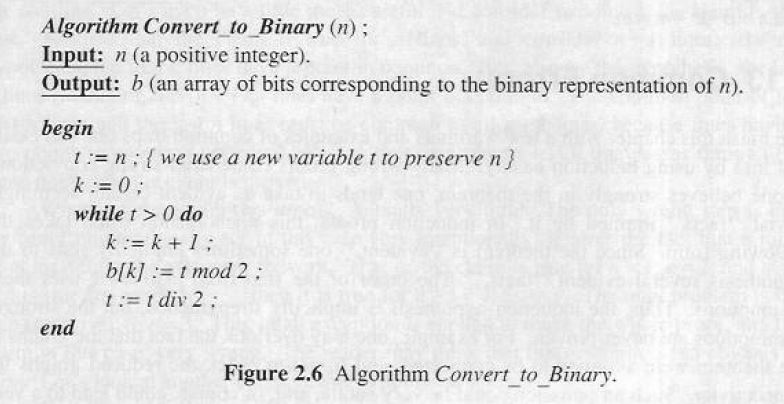
\includegraphics[scale = 0.6]{algo.jpg}}
\item For the following problem we will explore an induction and the
notion of an \textbf{invariant} of an algorithm, which put simply, is a statement about
a variable correct independent of the number of times a loop is executed. For the purposes of 
this algorithm the expression: $n = t \times 2^k + m$ is a loop invariant. Loop invariants can 
be hard to find but are often the heart of any algorithm.\\
\textbf{Induction Hypothesis: } if $m$ is the integer represented by 
the binary array $b[1\dots k]$, then $n = t \times 2^k + m$. To prove the 
correctness of this algorithm we must prove three conditions:
\begin{enumerate}
\item The hypothesis is true at the beginning of the loop.
\item The truth of the hypothesis at steps $k$ implies the step $k+1$.
\item When the loop terminates, the hypothesis implies the correctness of the algorithm.
\end{enumerate}
Attempt to complete the proof given the information I've given you to start. 
\end{enumerate}
\end{document}